%Tipo de Documento [Conferencia]

\documentclass[conference]{IEEEtran}\usepackage[]{graphicx}\usepackage[]{color}
%% maxwidth is the original width if it is less than linewidth
%% otherwise use linewidth (to make sure the graphics do not exceed the margin)
\makeatletter
\def\maxwidth{ %
  \ifdim\Gin@nat@width>\linewidth
    \linewidth
  \else
    \Gin@nat@width
  \fi
}
\makeatother

\definecolor{fgcolor}{rgb}{0.345, 0.345, 0.345}
\newcommand{\hlnum}[1]{\textcolor[rgb]{0.686,0.059,0.569}{#1}}%
\newcommand{\hlstr}[1]{\textcolor[rgb]{0.192,0.494,0.8}{#1}}%
\newcommand{\hlcom}[1]{\textcolor[rgb]{0.678,0.584,0.686}{\textit{#1}}}%
\newcommand{\hlopt}[1]{\textcolor[rgb]{0,0,0}{#1}}%
\newcommand{\hlstd}[1]{\textcolor[rgb]{0.345,0.345,0.345}{#1}}%
\newcommand{\hlkwa}[1]{\textcolor[rgb]{0.161,0.373,0.58}{\textbf{#1}}}%
\newcommand{\hlkwb}[1]{\textcolor[rgb]{0.69,0.353,0.396}{#1}}%
\newcommand{\hlkwc}[1]{\textcolor[rgb]{0.333,0.667,0.333}{#1}}%
\newcommand{\hlkwd}[1]{\textcolor[rgb]{0.737,0.353,0.396}{\textbf{#1}}}%

\usepackage{framed}
\makeatletter
\newenvironment{kframe}{%
 \def\at@end@of@kframe{}%
 \ifinner\ifhmode%
  \def\at@end@of@kframe{\end{minipage}}%
  \begin{minipage}{\columnwidth}%
 \fi\fi%
 \def\FrameCommand##1{\hskip\@totalleftmargin \hskip-\fboxsep
 \colorbox{shadecolor}{##1}\hskip-\fboxsep
     % There is no \\@totalrightmargin, so:
     \hskip-\linewidth \hskip-\@totalleftmargin \hskip\columnwidth}%
 \MakeFramed {\advance\hsize-\width
   \@totalleftmargin\z@ \linewidth\hsize
   \@setminipage}}%
 {\par\unskip\endMakeFramed%
 \at@end@of@kframe}
\makeatother

\definecolor{shadecolor}{rgb}{.97, .97, .97}
\definecolor{messagecolor}{rgb}{0, 0, 0}
\definecolor{warningcolor}{rgb}{1, 0, 1}
\definecolor{errorcolor}{rgb}{1, 0, 0}
\newenvironment{knitrout}{}{} % an empty environment to be redefined in TeX

\usepackage{alltt}

%BIBLIOTECAS

% Este paquete se utiliza para generar texto o graficas de relleno.
%\usepackage{blindtext, graphicx}
%Biblioteca para graficas
\usepackage{graphicx}
%Biblioteca para lectura de caracteres ortográficos (tildes..etc. ) 
\usepackage[utf8]{inputenc}
%Biblioteca para graficos vectrizados.svg 
\usepackage{svg}
\usepackage{enumerate}
%Biblioteca para enumerar figuras tablas.. etc en español 
\usepackage[spanish, es-tabla]{babel}


%INICIO DEL DOCUMENTO
\IfFileExists{upquote.sty}{\usepackage{upquote}}{}
\begin{document}


% TITULO DEL PAPER
\title{Analitica de transacciones en linea relacionadas con el conjunto de datos 
Online Retail}


% NOMBRE DE LOS AUTORES
\author{
  \IEEEauthorblockN{Raul Alejandro Buitrago Castellanos}
  %AUTOR 1	
  \IEEEauthorblockA{Universidad Distrital\\
  Francisco Jose de Caldas\\
  Bogota, Colombia\\
  Email: raulhabits@gmail.com}
 %\and
}

%TITULO
\maketitle

%Iniciar Abstract
\begin{abstract}
 Este documento continene un analisis del conjunto de datos denominado \textbf{\textit{Precios de Combustibles}} el cual fue obtenido del repositorio de datos abiertos de Colombia - www.datos.gov.co. Este analisis fue realizado con el fin de obtener informacion de las variaciones en los precios de los combustibles de acuerdo a diferentes variables en una linea de tiempo.
\end{abstract}
 

%Iniciar Palabras Clave Formato IEEE
\begin{IEEEkeywords}
	Conjunto de datos, mineria de datos, cientifico de datos, bigdata, inteligencia de negocios.
\end{IEEEkeywords}

%SECCIÓN 1. INTRODUCCIÓN 
\section{Introduccion}
 El análisis de datos representa un importante rol in la historia de la humanidad. Puede implementarse en diferentes ramas del conocimiento y en cualquier tipo de dato.\\
 Con el florecimiento de nuevas técnicas de datos y de la expansión y evolución sistemática en mejores motores de almacenamiento se ha generado un avance significativo en las diferentes técnicas y herramientas usadas en minería de datos como resultado natural de dicha evolución tecnológica.\\
 Las aplicaciones de las técnicas de análisis de datos son muy diversas debido a que se puede establecer medidas para ser analizadas en cualquier campo, como ejemplo en datos espaciales, datos de texto, multimedia, networking, WWW, inteligencia de negocios, análisis de ADN, entre otros.\\
 Entre todas las técnicas de análisis de datos son comúnmente usadas las estadísticas, el cálculo de probabilidades, técnicas de BigData, minería de datos y otras.

\section{Objetivos}
 Realizar un analisis estadistico, identificar las variables de mayor influencia, establecer comportamientos y/o patrones para predecir el comportamiento del mercado relacionado a las ventas en linea registradas en el conjunto de datos, utilizando tecnicas de mineria de datos y bigdata.
\section{Marco teorico}
 Para comprender en su totalidad los terminos que se mencionan en este documento es necesario conocer los siguientes terminos.
 
 \subsection{Estadistica}
 \subsection{Dataset o conjunto de datos}
 \subsection{Business intelligence o inteligencia de negocios}
 \subsection{Dataware house o bodega de datos}
 \subsection{Data mining o Mineria de datos}
 \subsection{Bigdata}
 \subsection{Machine learning}
\section{Estado del arte} 
Diferentes enfoques para  predicción de precios han implementado métodos como  árboles de decisión, regresión linear y clustering con resultados importantes.  Yang Lan Qin [11] usaron modelos de regresión lineal para predecir el precio de un filamento de poliéster como apoyo a la cadena de abastecimiento. Otras investigaciones usan técnicas de predicción de precios auto-adaptativos  algoritmos basados en Markov [12]. Para la predicción de costos de inventario se han usado algoritmos de minería de datos basados en redes neuronales y SVM (Support vector machine) [13]. Otros enfoques para la predicción del precio del té en el mercado usando el algoritmo RELIEF [14]. Para la predicción de los cargos a los tiquetes aéreos se han usado algoritmos multi-estratégia (Ripper, Q-Learning y series de tiempo ) de otras investigaciones [15]. También grafos basados en atributos han permitido la detección de fraudes en transferencia de precios  [16]. Con respecto a la predicción de indicadores del precio de gasolina se han usado diferentes técnicas de agrupamiento (clustering) [16] 

%SECCIÓN 3. METODOLOGIA
\section{Methodologia}
 El trabajo y analisis de datos de esta investigacion tiene las siguientes tareas.
 \begin{itemize}
  \item Reconocimiento de la informacion 
  \begin{itemize}
   \item Identificar el dominio
   \item Identificar el problema
   \item Objetivo SMART 
  \end{itemize}
  \item Analisis Exploratorio
  \item Analisis Multivariado
  \begin{itemize}
	\item Analisis de correlacion entre variables
  \end{itemize}
  \item Encontrar patrones
   \begin{itemize}
    \item Clustering
    \item Regresion lineal
   \end{itemize}  
  \item Conclusiones
 \end{itemize}

%SECCIÓN 3. PREGUNTAS INVESTIGACION
\section{Research Questions}
A correct investigation begins with the right questions, then an optimal definition of what else will be the proposal of the research. In this case these are the proposals.
 \begin{itemize}
  \item{Descriptive.}
  A descriptive question is used to identify and know the characteristics of the dataset.
  \begin{itemize}
   \item What's the min date of the measurement?
   \item What's the max date of the measurement?
   \item What's the product quantity sold in the measurement?
   \item What's the product quantity returned in the measurement?
  \end{itemize}
  \item{Exploratory.}
   An exploratory question consists in the searching of patterns or relations to support an investigation question.
  \begin{itemize}
   \item Which country bought the major products quantity in January of 2012?
   \item Which month had major sales?
   \item Which month had major devolutions?
   \item Which country had major sales?
   \item Which country had major devolutions?
  \end{itemize}
  \item{Inferential}
   An inferential question consists in the creation of an hypothesis to be solved analyzing the information.
  \begin{itemize}
   \item Was France the country with major sales in January of 2012?
  \end{itemize}
 \end{itemize}




\begin{itemize}
 \item Informacion sobre la cantidad de unidades involucradas en las transacciones.

% Table created by stargazer v.5.2 by Marek Hlavac, Harvard University. E-mail: hlavac at fas.harvard.edu
% Date and time: mar, abr 12, 2016 - 21:30:24
\begin{table}[!htbp] \centering 
  \caption{} 
  \label{} 
\begin{tabular}{@{\extracolsep{5pt}}lccccc} 
\\[-1.8ex]\hline 
\hline \\[-1.8ex] 
Statistic & \multicolumn{1}{c}{N} & \multicolumn{1}{c}{Mean} & \multicolumn{1}{c}{St. Dev.} & \multicolumn{1}{c}{Min} & \multicolumn{1}{c}{Max} \\ 
\hline \\[-1.8ex] 
cantidad & 232,959 & 9.410 & 242.464 & $-$80,995 & 80,995 \\ 
\hline \\[-1.8ex] 
\end{tabular} 
\end{table} 

 \item Informacion correspondiente al periodo de tiempo de la medicion
[1] "2010-01-12" "2011-12-10"
        Min.      1st Qu.       Median         Mean      3rd Qu. 
"2010-01-12" "2011-03-04" "2011-06-09" "2011-05-13" "2011-09-06" 
        Max. 
"2011-12-10" 

  
 \item Información correspondiente a los productos.

 
 \item Para conocer el producto mas vendido, se procede con una grafica que contiene la cantidad de productos por unidad vendidos
\begin{knitrout}
\definecolor{shadecolor}{rgb}{0.969, 0.969, 0.969}\color{fgcolor}
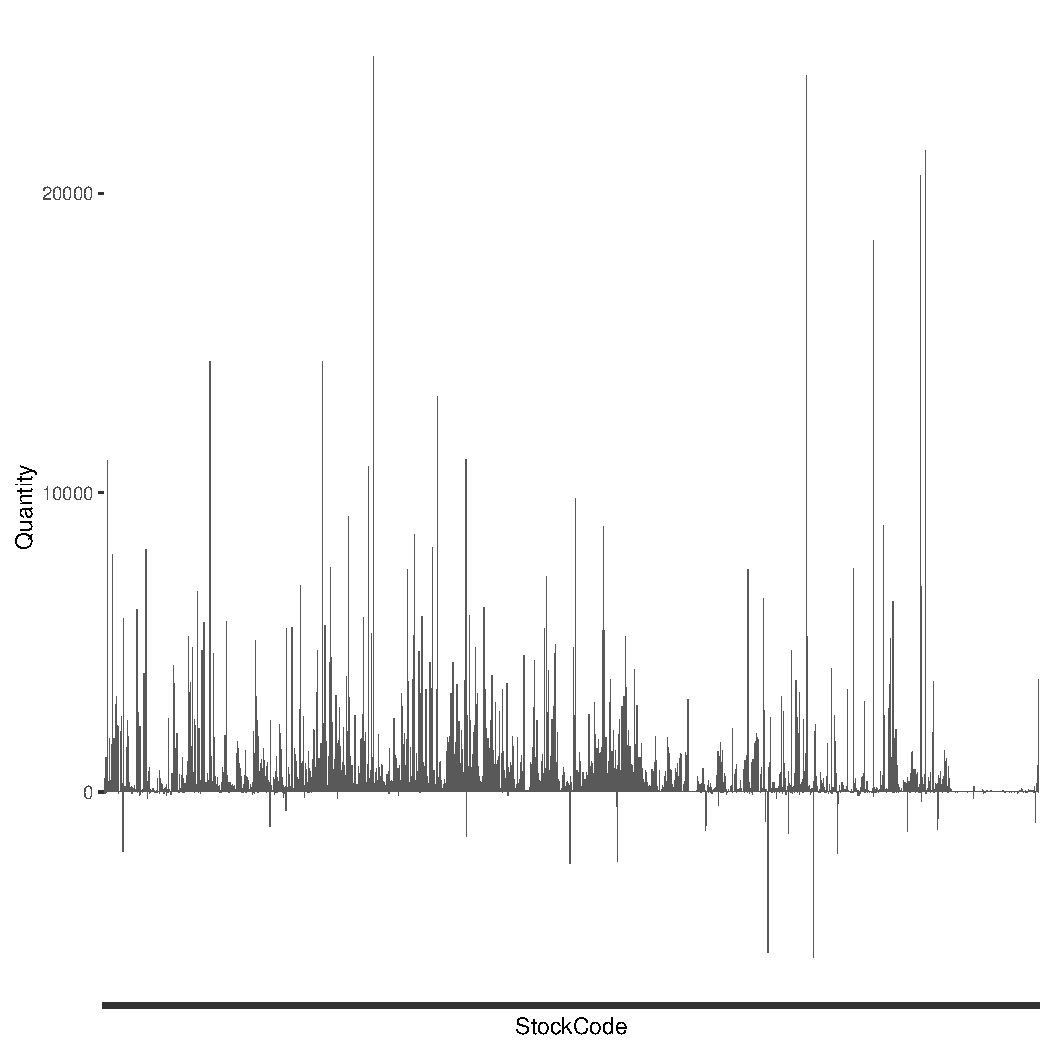
\includegraphics[width=\maxwidth]{figure/grafico_productos-1} 

\end{knitrout}

  \item Para conocer los registros de ventas de las transacciones se grafica la informacion de las transacciones mensuales
\begin{knitrout}
\definecolor{shadecolor}{rgb}{0.969, 0.969, 0.969}\color{fgcolor}
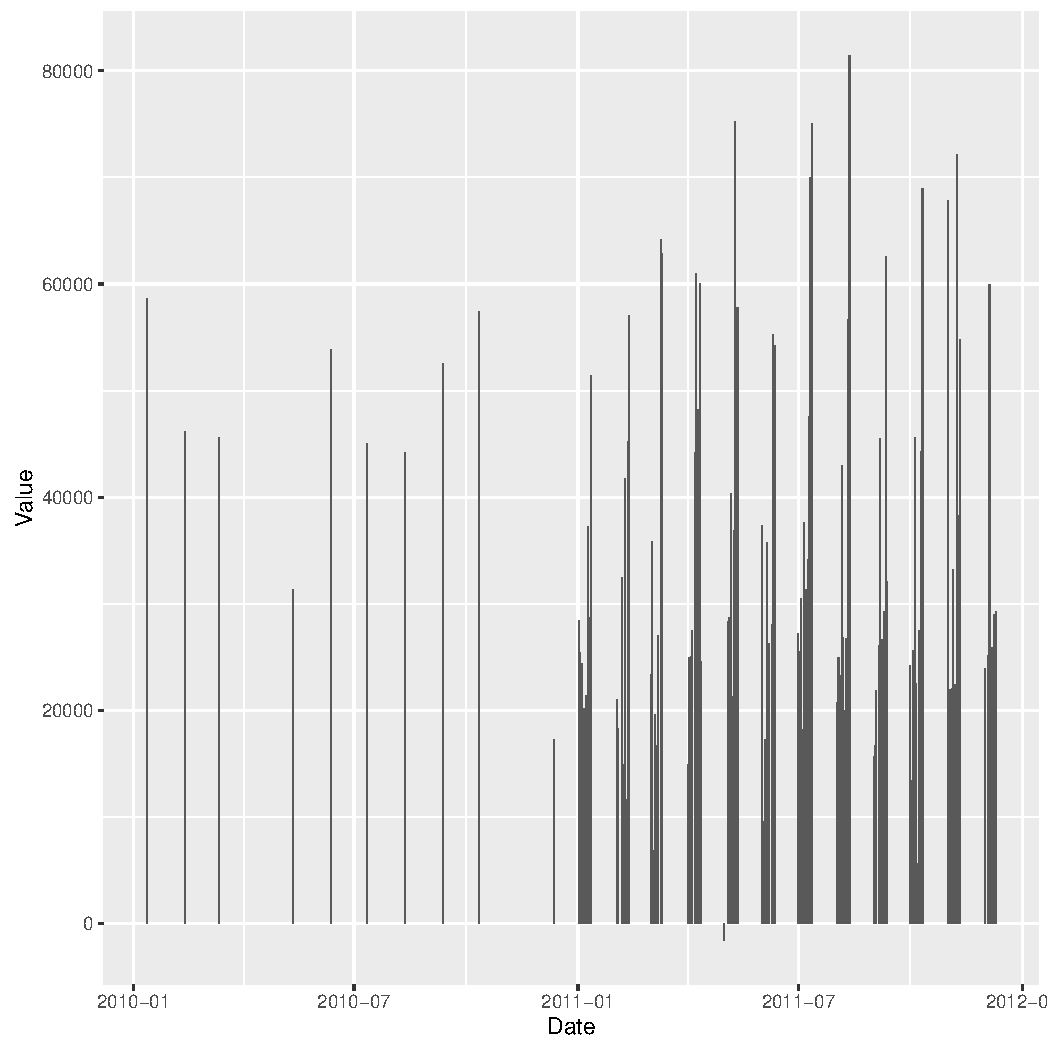
\includegraphics[width=\maxwidth]{figure/histograma_transacciones-1} 

\end{knitrout}
  
\end{itemize}





%BIBLIOGRAFÍA

%ENTORNO {thebibliography}
%Permite al autor listar las referencias utilizadas y citarlas en algun punto del texto.

\begin{thebibliography}{1}
		
	\bibitem{biblio1}
		B. Klaus and P. Horn, Robot Vision. Cambridge, MA: MIT Press, 1986. 
	\bibitem{biblio2}
		L. Stein, “Random patterns,” in Computers and You, J. S. Brake, Ed. New York: Wiley, 1994, pp. 55-70.
	\bibitem{biblio3}
		R. L. Myer, “Parametric oscillators and nonlinear materials,” in Nonlinear Optics, vol. 4, P. G. Harper and B. S.
	\bibitem{biblio4}
		Wherret, Eds. San Francisco, CA: Academic, 1977, pp. 47-160.
	\bibitem{biblio5}
		E. F. Moore, “Gedanken-experiments on sequential machines,” in Automata Studies (Ann. of Mathematical
	\bibitem{biblio5}
		Studies, no. 1), C. E. Shannon and J. McCarthy, Eds. Princeton, NJ: Princeton Univ. Press, 1965, pp. 129-153.
	\bibitem{biblio6}
		Westinghouse Electric Corporation (Staff of Technology and Science, Aerospace Div.), Integrated Electronic
	\bibitem{biblio7}
		Systems. Englewood Cliffs, NJ: Prentice-Hall, 1970. 

\end{thebibliography}

\end{document}
